The JSD-MP problem is NP-hard, so solving the ILP of
Section~\ref{sec:formulation} to optimality is intractable at the scale of a real
data center. In this section we propose MASMAN, a polynomial-time heuristic that
produces a near-optimal placement quickly enough to be used for admission control
on large infrastructures with many nodes and requests.

\subsection{Maximizing the Accepted SFC Requests with Management Constraints (MASMAN)}
Placing a chain involves two coupled sub-problems: \emph{VNF placement} (locating
the chain's VNFs) and \emph{VNFM placement} (locating the chain's manager). MASMAN
solves them in two phases, but keeps the first phase management-aware so that the
second phase rarely fails: before placement we reserve at least one VNFM's worth of
resources on every physical node, so a layout chosen in phase one cannot strand the
chain for lack of room to host its manager.

The first phase places the VNFs with the dynamic-programming algorithm of
Bari~\textit{et~al.}~\cite{Bari2015}. For each chain this algorithm finds a
minimum-cost placement by building a multi-stage graph---one stage per VNF of the
chain, with the candidate physical nodes as the vertices of each stage---and
running a Viterbi-style shortest-path recursion over it: the optimal placement up
to stage \(i\) at node \(n\) is obtained from the best placement at stage
\(i-1\), since a minimum-cost path is composed of minimum-cost sub-paths. The
original algorithm is management-blind; we make it management-aware by admitting a
candidate node at a stage only when, in addition to the VNF's compute and
bandwidth requirements, the reserved manager resources and the co-location
(\(\eta\)) and radius (\(\rho\)) constraints can still be satisfied for the
partial layout.

The second phase assigns each chain an admissible VNFM and then applies a Tabu
search to \emph{consolidate} managers and cut the license cost: it repeatedly
tries to merge the chains of one VNFM node onto another, accepting a merge when it
remains feasible and lowers the total license cost, while a tabu list prevents
re-examining recently tried node pairs. The two phases are detailed in
Algorithm~\ref{alg:masman}.

\begin{algorithm}
  \caption{MASMAN --- management-aware VNF placement (phase 1)}
  \label{alg:masman}
  \begin{algorithmic}[1]
    \Require{$chains$, $topology$}
    \Function{masman\_placement}{$chains, topology$}
    \ForAll{$chain \in chains$}
      \State{$L \gets len(chain)$}\Comment{number of VNFs in the chain}
      \State{$cost[\cdot,\cdot] \gets +\infty$;\quad $prev[\cdot,\cdot] \gets \textsc{nil}$}
      \ForAll{$n \in topology.nodes$}\Comment{stage 0: first VNF, no predecessor}
        \If{$hasEnoughResource(n, chain[0])$}
          \State{$cost[0, n] \gets nodeCost(n, chain[0])$}
        \EndIf
      \EndFor
      \For{$i \gets 1, L - 1$}\Comment{remaining stages}
        \ForAll{$n \in topology.nodes$}
          \ForAll{$k \in topology.nodes$}
            \If{$cost[i-1, k] < \infty$ \textbf{and} $feasible(i{-}1, k \rightarrow i, n)$}
              \State{$c \gets cost[i-1, k] + linkCost(k, n) + nodeCost(n, chain[i])$}
              \If{$c < cost[i, n]$}\Comment{keep the minimum-cost sub-path}
                \State{$cost[i, n] \gets c$;\quad $prev[i, n] \gets k$}
              \EndIf
            \EndIf
          \EndFor
        \EndFor
      \EndFor
      \State{$n^\star \gets \arg\min_{n} cost[L-1, n]$}
      \If{$cost[L-1, n^\star] < \infty$}\Comment{a feasible layout exists}
        \State{$reconstruct$ placement by following $prev$ from $(L{-}1, n^\star)$ back to stage 0}
        \State{$reserveResources(chain)$}
      \EndIf
    \EndFor
    \EndFunction
    \algstore{masman}
  \end{algorithmic}
\end{algorithm}
\begin{algorithm}
  \caption{MASMAN --- VNFM assignment and Tabu consolidation (phase 2)}
  \begin{algorithmic}[1]
    \algrestore{masman}
    \Function{masman\_manager\_placement}{$chains, topology, maxIterations$}
    \ForAll{$chain \in chains$}\Comment{initial feasible VNFM per chain}
      \ForAll{$n \in topology.nodes$}
        \If{$canBeManager(chain, n)$}\Comment{$\eta$, radius, capacity and resources for every VNF of the chain}
          \State{$chain.manager \gets n$;\quad $reserveManagementResources(n)$}
          \State{\textbf{break}}
        \EndIf
      \EndFor
    \EndFor
    \State{$tabu \gets \emptyset$;\quad $best \gets totalLicenseCost(chains)$}
    \For{$i \gets 1, maxIterations$}
      \State{$(n_1, n_2) \gets$ random distinct nodes with $(n_1, n_2) \notin tabu$}
      \State{$insert(tabu, (n_1, n_2))$ with the configured tenure}
      \If{$isMergePossible(n_1, n_2)$}\Comment{every chain on $n_1$ stays admissible on $n_2$}
        \State{move all chains with $manager = n_1$ to $n_2$}
        \State{$freeManagementResources(n_1)$;\quad $reserveManagementResources(n_2)$}
        \State{$cur \gets totalLicenseCost(chains)$}
        \If{$cur < best$}
          \State{$best \gets cur$}\Comment{accept the consolidating move}
        \Else
          \State{revert the move}\Comment{non-improving: undo, keep feasibility}
        \EndIf
      \EndIf
    \EndFor
    \EndFunction
  \end{algorithmic}
\end{algorithm}

\begin{figure}[h!]
  \centering
  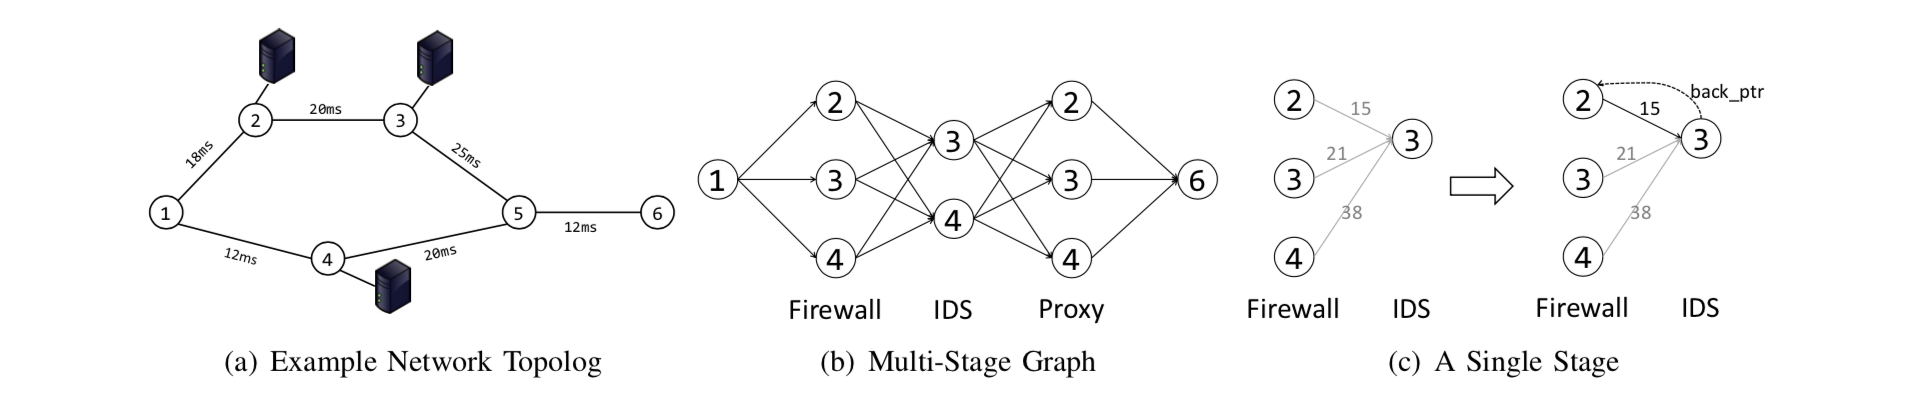
\includegraphics[width=\textwidth]{images/bari.png}
  \caption{Stage transitions of the \cite{Bari2015} algorithm used to build the
  multi-stage placement graph.}
\end{figure}

As a baseline for comparison, we also consider a management-blind variant that
runs the \cite{Bari2015} algorithm with an extra stage appended for the VNFM,
i.e. it places the manager only after the VNF layout is fixed. We use this
disjoint variant in Section~\ref{sec:results} to isolate the benefit of the
management-aware placement in Algorithm~\ref{alg:masman}.

\subsection{Complexity}
For a chain of \(L\) VNFs, the phase-one dynamic program fills an
\(L \times |V^p|\) table and evaluates each entry against every candidate
predecessor, so it costs \(O(L\,|V^p|^2)\) per chain and
\(O(|R|\,L_{\max}\,|V^p|^2)\) over all requests, where \(L_{\max}\) is the longest
chain. The feasibility test at each transition is dominated by a shortest-path
check on the management/service links, bounded by \(O(|E^p|)\). Phase two assigns
an initial manager in \(O(|R|\,|V^p|)\) and then runs \(maxIterations\)
consolidation steps, each \(O(|R|)\). The overall running time is therefore
polynomial in the size of the infrastructure and the request set, in contrast to
the exponential worst case of the exact ILP.
